\chapter{Realisierung des Source-To-Source Compilers}
\label{chap:Realisierung}
Gestützt auf das grundsätzliche Wissen über Compiler, die herausgearbeiteten Unterscheidungen von  Xamarin.Forms und Flutter sowie die Differenzen der verwendeten Programmiersprachen  \Csharp und Dart, wird in diesem Kapitel die Realisierung des Source-To-Source Compilers beschrieben.  Es bietet sich die \ac{ide} (deutsch Entwicklungsumgebung)(deutsch Entwicklungsumgebung) Visual Studio 2019 von Microsoft an,  um das Projekt mit Roslyn Integration zu implementieren,  denn auf dieser Plattform stehen Erweiterungen für Roslyn zur Verfügung.
Die zu entwickelnde Projektmappe,  besteht also aus dem Source to Source Compiler mit Rosyln Integration, der grafischen Benutzeroberfläche und einer Xamarin.Forms
Anwendung als Testobjekt,  wobei letzteres die jedoch erst im nächsten Kapitel genau eingeführt wird.


\section{Programmablauf}
Mithilfe des Roslyn Compilers kann der Source-To-Source Compiler Auswertungen zu den in der Xamarin.Forms App referenzierten Quelltextdateien durchführen.  Somit ist es
möglich eine Auflistung aller verfügbaren \Csharp - Dateien aus einem Projekt übergebenen Projekt zu extrahieren.  XAML -Dateien werden nicht von Roslyn behandelt.  Dies gelingt jedoch über den Umweg der Codebehind-Dateien mit Endung .XAML.CS,  die ein Laden über das Dateisystem ermöglichen. 

Nachdem der Source-To-Source Compiler alle Quelltext- und Ansichtsdateien übersetzt hat,  müssen die in Kapitel 4 beschriebenen Metadaten überführt werden.  Anschließend kann der Quelltext optimiert und der Übersetzungsvorgang abgeschlossen werden.  Folgend kann nun zur Visualisierung des Übersetzungsvorganges ein \ac{uml}  Aktivitätsdiagramm angelegt werden, wie es in Abbildung \ref{fig:umlablauf} dargestellt ist.

\newpage
\begin{figure}[!ht]
 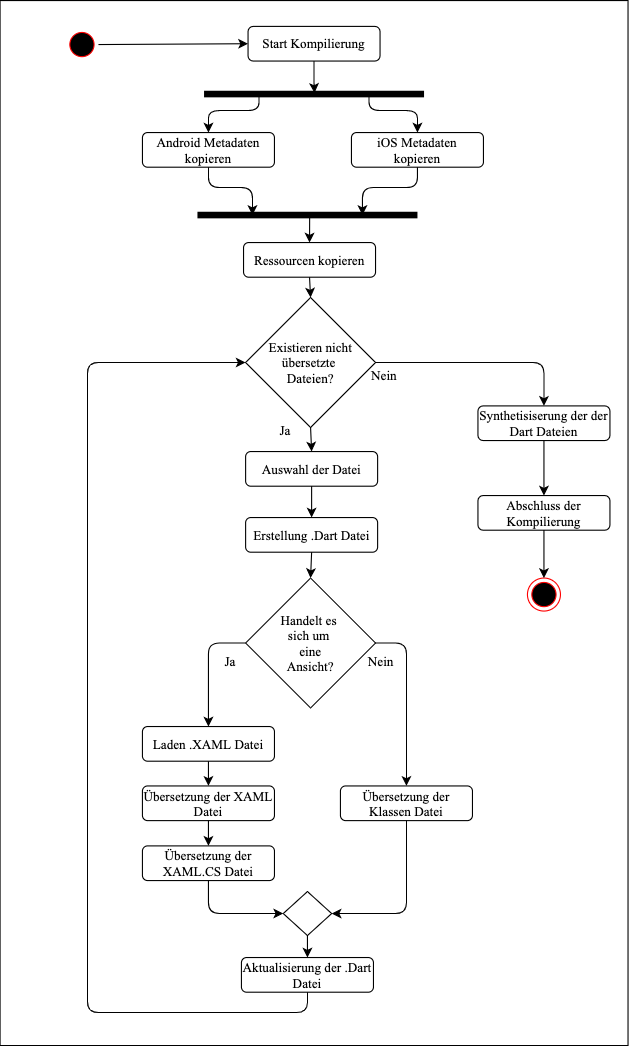
\includegraphics[width=\textwidth,keepaspectratio]{Images/Implementation/Ablauf.png}
 \caption{Aktivitätsdigramm}
 \label{fig:umlablauf}
\end{figure}

Das dargestellte \ac{uml}-Diagramm befindet sich aufgrund der Komplexität des Compilers auf einer hohen Abstraktionsebene. In den folgenden Abschnitten werden die einzelnen Aspekte der Kompilierung noch näher betrachtet.


\section{Metadaten}
Wie das UML Diagramm veranschaulicht können die Metadaten von Android und iOS parallel in die Flutter Anwendung kopiert werden.  Da die Metadaten
plattformspezifische Eigenschaften der mobilen Anwendungen sind, wird im nächsten Abschnitt auf die entsprechenden Details der beiden Betriebssysteme eingegangen.


\subsection{Android Metadaten}
Zu den Android spezifischen Metadaten gehören die sogenannten Launcher Icons, die den Anwendern als App-Icon angezeigt werden. Xamarin.Android speichert dieses grafische Symbol in Ordnern, die die unterschiedlichen Pixeldichten der Android-Geräte unterstützen und in denen unter Umständen auch andere Bilder gespeichert sind.  Innerhalb von Xamarin.Forms wird das ausgewählte Icon über die Klasse MainActivity.cs definiert, wie dies in Quelltext \ref{lst:IconName} dargestellt ist. 

\lstinputlisting[label={lst:IconName},caption={Xamarin.Forms Android Launcher-Icon Name}, language=csh]{SourceCode/IconName.cs}

Nach der Extraktion des Namens können nun die Bilder kopiert werden.  In der durch die Flutter SDK erzeugten App liegen bereits Bildplatzhalter zum Austausch bereit.

Der eindeutige Identifizierer, PackageID,  zählt ebenfalls zu den Metadaten und Identifiziert die  Anwendungen auf dem mobilen Gerät und im GooglePlay Store.  Die Information über die ID kann in Xamarin.Forms aus der AndroidManifest.XML Datei ausgelesen  werden, und muss aber in Flutter sowohl in 3 Manifest Dateien als auch in die build.gradle geschrieben werden.Das Plugin,  change\_app\_package\_name , nimmt alle notwendigen Änderungen vor. Es muss als Abhängigkeit zum Projekt hinzugefügt und anschließend über die Kommandozeile ausgeführt werden. 


Der Anwendungsnamen wird, wie die Package ID, aus dem AppManifest extrahiert, und in Flutter allerdings auch nur in eine Manifest Datei geschrieben, wobei ausschließlich die Datei im 
Verzeichnis ’Project/app/src/main’ aktualisiert werden muss.

Ein weiterer Inhalt des AppManifests sind die Berechtigungen, welche die mobile Anwendung während der Laufzeit erfragen kann. Diese können ebenfalls wie der Name
kopiert werden. 

\subsection{iOS Metadaten}
Bei iOS werden die weiter oben beschriebenen Metadaten alle innerhalb der Info.Plist Datei verwaltet.  Jedoch werden in dieser Datei innerhalb des Flutter Projektes teilweise Variablen für die entsprechenden Information geladen die in der AppFrameworkInfoPlist gespeichert werden.  Zu diesen Informationen gehören die Buildnummer und der Identifizierer der Anwendung.  Damit die Anwendung nach der Kompilierung zu einer Flutter App genau so zu administrieren ist, wie eine normale Flutter Anwendung soll dieses Schema Beibehalten werden.  Daher werden die entsprechenden Einträge aus der Info.Plist extrahiert und jeweils in die Info.Plist Dateien von Flutter kopiert. 
Für das AnwendungsIcon kann das Verzeichnis Assets.xcassets aus dem Stammverzeichnis der Xamarin.Forms iOS App in das Verzeichnis ios/flutter/Runner kopiert werden.  Dieses beinhaltet alle notwendigen Icons.


\subsection{Ressourcen}
Neben diesen Metadaten müssen auch weitere Ressourcen kopiert werden.  Dazu gehören die Bilder die innerhalb der Anwendung angezeigt werden und bei Xamarin.Forms üblicherweise innerhalb der plattformspezifischen Anwendungen abgelegt werden.  Der in dieser Arbeit realisierte Compiler kopiert die Bilder aus dem iOS Verzeichnis der Xamarin.Forms Anwendung für die spätere Verwendung in der Flutter App.  Dies hat jedoch zur Folge, dass bei der Verwendung von unterschiedlichen Bildern je nach Plattform die Android Varianten nicht übernommen werden.  Um diese Bilder anzeigen zu können werden innerhalb der Flutter App im Verzeichnis Assets zwei Unterodner mit den Namen 2.0x und 3.0x angelegt, welche für die Speicherung von höheraufgelösten Bilder verwendet werden.  Bilder mit der Endung @2x werden anschließend in das 2.0x verzeichnis und 3@x Bilder in das Verzeichnis 3.0x abgelegt.  Dateien ohne entsprechende Endung werden einfach im Asset Verzeichnis abgelegt.  Neben dieser Kopie der Bilder ist es auch notwendig,  die Ressourcen innerhalb der pubspec.yaml zu referenzieren. Ähnlich werden die Customfonts behandelt,  sie werden aus dem iOS Vereichnis kopiert und anschließend in der pubspec.yaml Datei hinzugefügt.  


Die Startbildschirme der Anwendung sind essentiell,  da eine Anwendung ohne diese nicht in den Appstore aufgenommen wird.  Da diese Ansicht angezeigt wird,  während die App geladen wird sind diese meist simple aufgebaut um keine zusätzliche Ladezeit zu generieren.  Die generierte Flutter Anwendung beinhaltet für jede Plattform automatisch einen Startbildschirm der wiederverwendet werden kann.  Folglich verwendet der Compiler definierte Icons der Xamarin.Forms Plattformen und kopiert diese an die entsprechenden Stellen innerhalb der Flutter Anwendung.  



\section{Übersetzung von Klassenstrukturen}

Die Übersetzung von \Csharp zu Dart ist ein essentieller Bestandteil des Compilers.  Dafür wird zuerst die Visual Studio Projektmappe,  welches das Xamarin.Forms Projekt beinhaltet geladen.  Anschließend wird das Projekt, welches den gemeinsamen Quelltext beinhaltet weiter betrachtet. Da in dieser Arbeit kein plattformspezifischer Quelltext betrachtet wird,  werden diese Projekte ausschließlich für das Kopieren der Metadaten benötigt.  Anschließend kann für jede Klasse innerhalb des geteilten Projekts die Syntaxanalyse durchgeführt werden, welche den Syntaxbaum zurückliefert.  Darauf aufbauend wird das sogenannte semantische Model generiert.  Dieses semantische Model speichert Symbole der Source-Code Klasse innerhalb der Symboltabelle.  Diese schritte beschreiben das Compiler-Frontend und werden von Roslyn ebenfalls bei der Kompilierung von Projekten zu ausführbaren Dateien umgesetzt.  
<Beschreibung Arbeitsweise Übersetzer>

Modifizierer
Austausch von Typen

Wie in Kapitel 4 beschrieben werden viele Funktionalitäten mithilfe von Erweiterungen realisiert.  Jedoch sind die Erweiterungen, wenn auch vergleichbar, von anderen Herstellern mit unterschiedlichen Anforderungen realisiert worden.  Dies führt dazu,  dass Klassen und Methoden aus diesen Bibliotheken keine identischen Repräsentationen sind.  Diese Inkompatibilität kann nicht mittels Automation gelöst werden und Bedarf  unterschiedlich umfangreicher manueller Umwandlungen.  


\section{Übersetzung von Ansichten}
Die Übersetzung von Ansichten inkludiert die XAML und XAML.Cs Dateien, die anschließend in einer gemeinsamen Dart-Datei synthetisiert werden müssen.  Daraus folgt,  das für beide Typen von Ursprungsdateien jeweils ein Compiler Front-End,  welches die Aufgaben bis zur Zwischendarstellung übernimmt entwickelt werden musste.  Basierend auf den beiden Zwischendarstellungen kann anschließend in einem gemeinsamen Compiler-Backend die Zusammenführung sowie die Code-Optimierung durchgeführt werden.  Dies wird in Abbildung  \ref{fig:ViewCompilerPhases} visualisiert. 

\begin{figure}[!ht]
 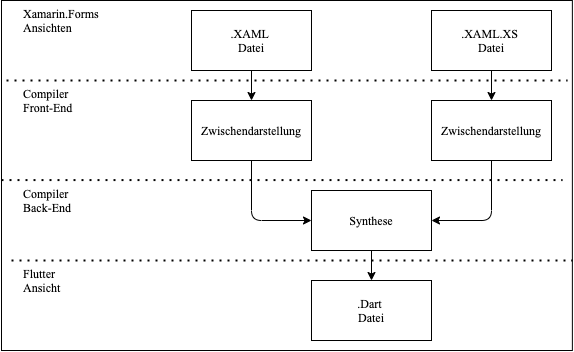
\includegraphics[width=\textwidth,keepaspectratio]{Images/Implementation/ViewCompiler.png}
 \caption{Compiler Phasen für Ansichten}
 \label{fig:ViewCompilerPhases}
\end{figure}

\subsection{Visuellen- Zwischendarstellung}

Für die visuelle Zwischendarstellung wird in einem ersten Schritt die XML Struktur aus der XAML Datei ausgelesen und basierend auf dieser Struktur ein Syntaxbaum mitsamt der Eigenschaften der einzelnen Elemente angelegt.  Mit Hilfe des .Net Frameworks kann die XML Struktur der XAML-Datei durchlaufen und analysiert werden.  Dafür wurde das in Abbildung \ref{fig:Klassendiagram} dargestellte Klassendiagramm entworfen. 
\newpage

\begin{figure}[!ht]
 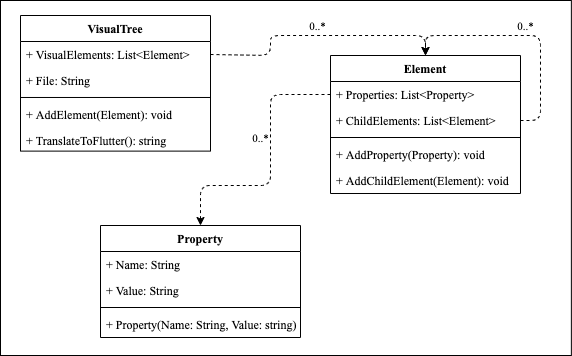
\includegraphics[width=\textwidth,keepaspectratio]{Images/Implementation/Klassendiagram.png}
 \caption{Klassendiagram}
 \label{fig:Klassendiagram}
\end{figure}

Anschließend stellt ein Objekt der Klasse VisualTree den Layout-Baum einer speziellen XAML Datei dar.  Er beinhaltet eine Auflistung von untergeordneten Elemten, welche wiederum weitere Elemente beinhalten können um die Verschachtelung des Baumes abzubilden. Darüber hinaus hat jedes Element eine Auflistung von Eigenschaften welche die Attribute der einzelnen XML Knoten beschreiben.  Basierend auf diesem Baum wird anschließend basierend auf den in Kapitel 4 beschriebenen Gegenüberstellungen von Flutter Widgets ein Austausch von den visuellen Elementen durchgeführt.  Dabei wird für jedes Widget der Quelltext zur Initialisierung in einem Template vorgehalten.  Alle möglichen Variablen und Eigenschaften dieser Widgets werden innerhalb dieser Vorlagen mit Platzhaltern bereitgestellt.  Dies wird in Quelltext \ref{st:Placeholder} dargestellt.

\lstinputlisting[label={lst:Placeholder},caption={Exemplarische LoginPage in Dart} , language=Dart]{SourceCode/DartPlaceholder.dart} 

Einige dieser Platzhalten können in einem nächsten Schritt ersetzt werden.  Dafür müssen die jeweiligen Werte aus den Eigenschaften der Xamarin Forms Elemente extrahiert und anschließend in das Template eingetragen werden.  Jedoch gibt es auch Variablen die entweder nicht angegeben oder mithilfe eines Bindings über die Codebehind Datei gesetzt werden.   

\subsection{Logische- Zwischendarstellung}
Die Erzeugung der logischen Zwischendarstellung verwendet für die Übersetzung des \Csharp Quelltextes den gleichen Übersetzter der auch schon für die Übersetzung von Klassenstrukturen verwendet wurde,  da es sich bei diesen Dateien ausschließlich um \Csharp Klassen handelt.  Für die Aktualisierung der Benutzeroberfläche ist es jedoch auch notwendig. erweiterte Änderungen vorzunehmen.  Bei Xamarin.Forms werden Änderungen an Eigenschaften automatisch an die Benutzeroberfläche übermittelt. Dies ist bei Flutter nicht der Falle,  stattdessen muss mit Hilfe der setState()) Methode das Framework über eine Veränderung informiert werden.  Die notwendige Änderung am Quelltext kann nicht bei der Erstellung der Zwischendarstellung geschehen, da aus sicht der Codebhind Datei nicht ermittelbar ist,  welche Eigenschaften eine direkten Bezug zur Ansicht haben. 


\subsection{Compiler Backend}
Das Compiler Backend beinhaltet die Synthetisierung bei der die beiden einzelnen Zwischendarstellungen zusammengeführt werden.  Dafür werden die gesamten Methoden und Eigenschaften aus der logischen Darstellung in die Ansicht überführt und die Referenzierungen in der Ansicht entsprechend angepasst.  Zu diesem Zeitpunkt ist es möglich,  zu ermitteln welche Eigenschaften und Methoden im \ac{ui} zu Veränderungen führen.  Stellen im Quelltext wo diese Veränderungen durchgeführt werden müssen folglich in einen SetState Block eingefügt werden,  damit Änderungen automatisch auf der Oberfläche der App angezeigt werden.

<Algorithmus Zusammenführung>


Nach der erfolgreichen Synthetisierung kann die Codeoptimierung durchgeführt werden.  Hierbei ist es wichtig die noch vorhandenen Platzhalter im Quelltext zu entfernen damit dieser einen korekten Syntaktischen Zustand einnimmt.  Folglich kann die mobile App nach diesem Vorgang ausgeführt werden. 

<Algorithmus Optimierung>


\section{Grafische Benutzeroberfläche}
Die GUI ist der zentrale Berührungspunkt von Anwendern mit dem Transpiler.  Sie soll die notwendigen Eingabe-Möglichkeiten anbieten, das Ergebnis ausgeben und den Anwender auf mögliche Fehler hinweisen.  Das grafische Vorbild ist das in Kapitel 3 entworfene Mockup, siehe Abbildung 3.4.  Für die Erstellung einer entsprechenden Benutzeroberfläche stehen eine Vielzahl von Technologien. Mit verschiedenen Vor- und Nachteilen zur Verfügung.  Eine Webseite wäre von Vorteil, da Anwender keinen Installationsaufwand hätten und  plattformunabhängig auf den Compiler zugreifen könnten.  Allerdings ist zumindest ein gewisser Kontrollverlust über den eigenen Quelltext durch das  Hochladen auf eine Webseite nicht ausgeschlossen.  Die Bedienoberfläche dieser Arbeit soll daher eine lokale Anwendung sein, sodass kein  unberechtigter Zugriff auf den Source-Code des Anwenders möglich ist. Zu diesem Zwecke wird die GUI mit der Technologie \ac{wpf}  realisiert. Dabei handelt es sich um ein UI-Framework des .NET Frameworks, das welches für die Erstellung von Desktopanwendungen geeignet ist und mit XAML und \Csharp entwickelt wird. \footcite[Vgl.][S. 1f]{Wenger2012} 

Anwendungen die mittels WPF programmiert werden, sind nur unter Windows als Betriebssystem  ausführbar.  Da diese Festlegung auf Windows bereits durch Build Tools erfolgte, entstehen hier  keine zusätzlichen Einschränkungen. Eine Web-Oberfläche des Source to Source Compilers hätte, im Gegensatz zu der aktuellen  Implementierung, durchaus auch Vorteile und könnte für die Zukunft ein Modell darstellen.  Es würde sich der Installationsaufwand reduzieren und die Installation könnte von der 
Anzeige entkoppelt werden. Die Plattformunabhängigkeit von Webseiten bietet einen weiteren Pluspunkt,  da 
Xamarin.Forms Entwickeler mit einem Mac OSX Computer könnten ebenfalls vom Compiler  profitieren, da eine Windows Installation entfällt.

<Screenshot Anwendung >

Da sowohl die grafische Benutzeroberfläche als auch der Source-To-Source Compiler mit .Net Technologien realisiert wurden lassen sie sich einfach miteinander kombinieren.  Dafür wird der Compiler als Ahängigkeit in das Projekt der grafischen Benutzeroberfläche geladen.

\section{Zusammenfassung}
In diesem Kapitel wurde beschrieben, wie der Source-To-Source Compiler entwickelt wurde.  Während der Realisierung wurden Entscheidungen getroffen,  die dafür sorgen das Xamarin.Forms und Flutter Anwendung nicht vollständig identisch sind.  Zum einen wurden die Bilder, die innerhalb der Anwendung angezeigt werden ausschließlich aus dem iOS Projekt entnommen,  zum anderen werden die Startbildschirme der nativen Xamarin.Forms Anwendungen nicht vollständig übernommen sondern ausschließlich das anzuzeigende Bild. 
